\chapter{Metodologia}\label{ch:metodologia}

Este capítulo apresenta os procedimentos e métodos adotados para a realização do projeto. Aqui serão detalhados o tipo e a abordagem da pesquisa, o contexto no qual o estudo se encontra, a população e a amostra analisadas, e por fim as técnicas de coleta e análise de dados utilizadas.

\section{Tipo e Abordagem de Pesquisa}

Este projeto consiste de uma pesquisa aplicada e exploratória, visando compreender melhor o tema de linguagem de programação baseada em ECS, que ainda é pouco abordado, e assim prover um protótipo com aplicações práticas como base para pesquisas futuras.

O projeto busca investigar o \textit{design} e a implementação da linguagem com uma abordagem focada em aspectos qualitativos, como usabilidade, modularidade e segurança, descartando qualquer aspecto quantitativo, como o desempenho. Essa abordagem será aplicada no estudo e análise de todas as etapas do projeto, desde a definição do \textit{design} da linguagem até a implementação do protótipo de interpretador.

\section{Contexto}

O projeto se encontra no contexto dado pela intersecção da área de desenvolvimento de linguagens de programação e do padrão arquitetural \textit{Entity Component System} (ECS). O ECS guia o \textit{design} e a implementação da linguagem de programação proposta de forma a facilitar o uso do padrão.

\section{Delimitação do Estudo}

Com a finalidade de manter o foco do projeto em seus objetivos centrais, serão estabelecidas algumas delimitações. O escopo do \textit{design} e da implementação do projeto estará estritamente concentrado na linguagem de programação e em sua biblioteca padrão (do inglês, \textit{standard library}).

Dessa forma, o projeto não abordará aspectos relacionados ao ecosistema de desenvolvimento, como \textit{syntax highlighting} e \textit{Language Server Protocol} (LSP).

\section{População e Amostra}

A população de referência para o estudo são linguagens de programação e bibliotecas que implementam ou dão suporte ao padrão ECS. A amostra escolhida inclui a linguagem Rust e as bibliotecas de ECS Flecs e Bevy, por serem extremamente relevantes no contexto de ECS e por serem inovadoras em suas abordagens.

\section{Técnicas de Coleta de Dados}

Para a coleta de dados, foram utilizadas as técnicas de pesquisa bibliográfica, documental e experimental, conforme descrito a seguir:

\begin{itemize}
    \item \textbf{Pesquisa Bibliográfica}: análise de livros, artigos e publicações acadêmicas sobre linguagens de programação, ECS e \textit{design} de software;
    \item \textbf{Pesquisa Eocumental}: análise de documentação, repositórios de código-fonte e exemplos de uso de linguagens e bibliotecas que implementam o padrão ECS;
    \item \textbf{Pesquisa Experimental}: definição do \textit{design} da linguagem de forma iterativa com base na análise qualitativa dos resultados.
\end{itemize}

\section{Técnicas de Análise de Dados}

A análise dos dados coletados será realizada de forma qualitativa, por meio das seguintes técnicas de análise:

\begin{itemize}
    \item \textbf{Análise Documental e Bibliográfica}: análise e interpretação dos conceitos, padrões e práticas encontrados nas fontes pesquisadas.
    \item \textbf{Análise Comparativa}: avaliação das características do protótipo em comparação com linguagens e bibliotecas selecionadas na amostra, destacando pontos fortes e limitações.
\end{itemize}

\section{Procedimentos Metodológicos}

O procedimento metodológico adotado para o desenvolvimento deste trabalho será dividido em etapas auto-contidas, ou seja, cada etapa será realizada de forma independente, mas todas interligadas para alcançar o objetivo final do projeto. As etapas são as seguintes:

\begin{enumerate}
    \item \textbf{MVP Fundacional da Linguagem}: inclui os conceitos de entidade, componente e sistema, representando um mínimo produto viável (do inglês, \textit{minimum viable product} — MVP). A conclusão desta etapa não segere uma linguagem pronta para uso prático, mas sim um protótipo funcional que pode ser utilizado para provar a viabilidade da fundação do trabalho;
    \item \textbf{Operações Envolvendo Entidades}: inclui as operações essenciais da linguagem, como a criação e remoção de entidades, além da adição e remoção de componentes.
    \item \textbf{Inserção de Componentes em Tempo de Compilação}: inclui a operação de inserção de componentes em entidades durante o tempo de compilação. Esta etapa é essencial para a etapa seguinte, que fará uso da operação implementada nesta;
    \item \textbf{Agendamento de Sistemas}: inclui o agendamento de sistemas, permitindo que o programador defina a ordem de execução deles. Esta etapa fará uso da operação de inserção de componentes em tempo de compilação implementada na etapa anterior;
    \item \textbf{\textit{Querying} de Entidades}: inclui a operação de \textit{querying} de entidades dentro de sistemas, permitindo que o programador consulte entidades com base em seus componentes. Esta é a etapa final do projeto, onde todos os conceitos terão sido implementados e analisados.
\end{enumerate}

Todas as etapas do trabalho serão compostas de três subetapas cronológicas: planejamento, implementação e análise, respectivamente. Elas são descritas a seguir:

\begin{enumerate}
    \item \textbf{Planejamento}: consiste na definição dos objetivos e \textit{design} dos conceitos relacionados a etapa, incluindo a definição de sintaxe e semântica;
    \item \textbf{Implementação}: consiste na implementação dos conceitos relacionados a etapa, sempre levando em consideração a linguagem como um todo;
    \item \textbf{Análise}: consiste na análise qualitativa do \textit{design} definido usando as características e critérios definidos na \autoref{sec:design_linguagem}, além de uma análise comparativa com as bibliotecas de ECS selecionadas na amostra. O processo de implementação também será analisado, buscando documentar possíveis problemas e soluções encontradas.
\end{enumerate}

A motivação por trás dessa escolha de metodologia é dada pela possibilidade de gerar um MVP logo na primeira etapa do trabalho, gerando \textit{feedback} fundacional para o restante do trabalho. Além disso, a abordagem iterativa permite uma evolução incremental, permitindo ajustes e melhorias ao longo do desenvolvimento.

A \autoref{fig:diagrama_geral} apresenta o diagrama geral do protótipo de interpretador proposto pelo trabalho.

\begin{figure}[H]
	\centering
	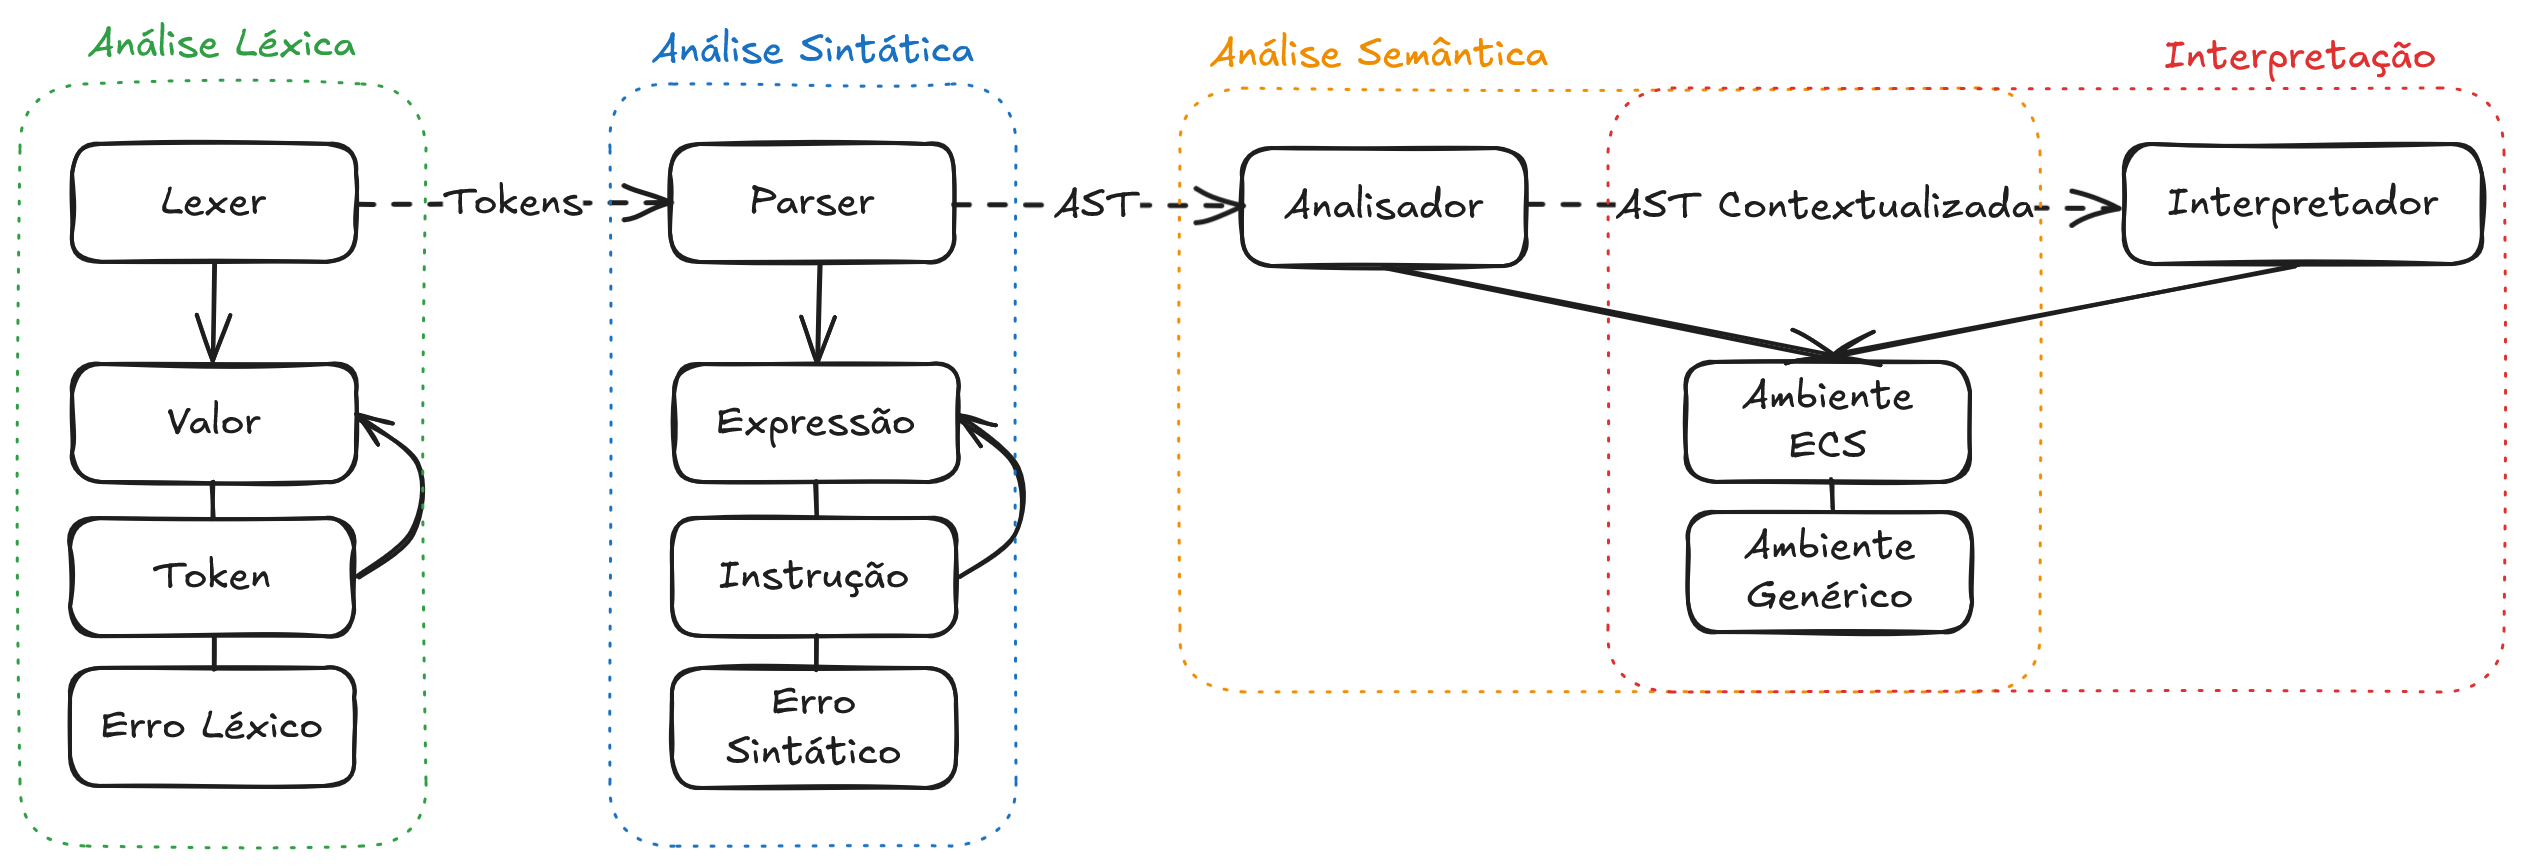
\includegraphics[width=0.65\textheight]{diagrama_geral.excalidraw.png}
	\caption{Diagrama geral do protótipo de interpretador.}
	\fonte{Elaboração própria.}
	\label{fig:diagrama_geral}
\end{figure}
